% Options for packages loaded elsewhere
\PassOptionsToPackage{unicode}{hyperref}
\PassOptionsToPackage{hyphens}{url}
%
\documentclass[
]{article}
\usepackage{amsmath,amssymb}
\usepackage{lmodern}
\usepackage{ifxetex,ifluatex}
\ifnum 0\ifxetex 1\fi\ifluatex 1\fi=0 % if pdftex
  \usepackage[T1]{fontenc}
  \usepackage[utf8]{inputenc}
  \usepackage{textcomp} % provide euro and other symbols
\else % if luatex or xetex
  \usepackage{unicode-math}
  \defaultfontfeatures{Scale=MatchLowercase}
  \defaultfontfeatures[\rmfamily]{Ligatures=TeX,Scale=1}
\fi
% Use upquote if available, for straight quotes in verbatim environments
\IfFileExists{upquote.sty}{\usepackage{upquote}}{}
\IfFileExists{microtype.sty}{% use microtype if available
  \usepackage[]{microtype}
  \UseMicrotypeSet[protrusion]{basicmath} % disable protrusion for tt fonts
}{}
\makeatletter
\@ifundefined{KOMAClassName}{% if non-KOMA class
  \IfFileExists{parskip.sty}{%
    \usepackage{parskip}
  }{% else
    \setlength{\parindent}{0pt}
    \setlength{\parskip}{6pt plus 2pt minus 1pt}}
}{% if KOMA class
  \KOMAoptions{parskip=half}}
\makeatother
\usepackage{xcolor}
\IfFileExists{xurl.sty}{\usepackage{xurl}}{} % add URL line breaks if available
\IfFileExists{bookmark.sty}{\usepackage{bookmark}}{\usepackage{hyperref}}
\hypersetup{
  pdftitle={semana 1},
  pdfauthor={luis},
  hidelinks,
  pdfcreator={LaTeX via pandoc}}
\urlstyle{same} % disable monospaced font for URLs
\usepackage[margin=1in]{geometry}
\usepackage{color}
\usepackage{fancyvrb}
\newcommand{\VerbBar}{|}
\newcommand{\VERB}{\Verb[commandchars=\\\{\}]}
\DefineVerbatimEnvironment{Highlighting}{Verbatim}{commandchars=\\\{\}}
% Add ',fontsize=\small' for more characters per line
\usepackage{framed}
\definecolor{shadecolor}{RGB}{248,248,248}
\newenvironment{Shaded}{\begin{snugshade}}{\end{snugshade}}
\newcommand{\AlertTok}[1]{\textcolor[rgb]{0.94,0.16,0.16}{#1}}
\newcommand{\AnnotationTok}[1]{\textcolor[rgb]{0.56,0.35,0.01}{\textbf{\textit{#1}}}}
\newcommand{\AttributeTok}[1]{\textcolor[rgb]{0.77,0.63,0.00}{#1}}
\newcommand{\BaseNTok}[1]{\textcolor[rgb]{0.00,0.00,0.81}{#1}}
\newcommand{\BuiltInTok}[1]{#1}
\newcommand{\CharTok}[1]{\textcolor[rgb]{0.31,0.60,0.02}{#1}}
\newcommand{\CommentTok}[1]{\textcolor[rgb]{0.56,0.35,0.01}{\textit{#1}}}
\newcommand{\CommentVarTok}[1]{\textcolor[rgb]{0.56,0.35,0.01}{\textbf{\textit{#1}}}}
\newcommand{\ConstantTok}[1]{\textcolor[rgb]{0.00,0.00,0.00}{#1}}
\newcommand{\ControlFlowTok}[1]{\textcolor[rgb]{0.13,0.29,0.53}{\textbf{#1}}}
\newcommand{\DataTypeTok}[1]{\textcolor[rgb]{0.13,0.29,0.53}{#1}}
\newcommand{\DecValTok}[1]{\textcolor[rgb]{0.00,0.00,0.81}{#1}}
\newcommand{\DocumentationTok}[1]{\textcolor[rgb]{0.56,0.35,0.01}{\textbf{\textit{#1}}}}
\newcommand{\ErrorTok}[1]{\textcolor[rgb]{0.64,0.00,0.00}{\textbf{#1}}}
\newcommand{\ExtensionTok}[1]{#1}
\newcommand{\FloatTok}[1]{\textcolor[rgb]{0.00,0.00,0.81}{#1}}
\newcommand{\FunctionTok}[1]{\textcolor[rgb]{0.00,0.00,0.00}{#1}}
\newcommand{\ImportTok}[1]{#1}
\newcommand{\InformationTok}[1]{\textcolor[rgb]{0.56,0.35,0.01}{\textbf{\textit{#1}}}}
\newcommand{\KeywordTok}[1]{\textcolor[rgb]{0.13,0.29,0.53}{\textbf{#1}}}
\newcommand{\NormalTok}[1]{#1}
\newcommand{\OperatorTok}[1]{\textcolor[rgb]{0.81,0.36,0.00}{\textbf{#1}}}
\newcommand{\OtherTok}[1]{\textcolor[rgb]{0.56,0.35,0.01}{#1}}
\newcommand{\PreprocessorTok}[1]{\textcolor[rgb]{0.56,0.35,0.01}{\textit{#1}}}
\newcommand{\RegionMarkerTok}[1]{#1}
\newcommand{\SpecialCharTok}[1]{\textcolor[rgb]{0.00,0.00,0.00}{#1}}
\newcommand{\SpecialStringTok}[1]{\textcolor[rgb]{0.31,0.60,0.02}{#1}}
\newcommand{\StringTok}[1]{\textcolor[rgb]{0.31,0.60,0.02}{#1}}
\newcommand{\VariableTok}[1]{\textcolor[rgb]{0.00,0.00,0.00}{#1}}
\newcommand{\VerbatimStringTok}[1]{\textcolor[rgb]{0.31,0.60,0.02}{#1}}
\newcommand{\WarningTok}[1]{\textcolor[rgb]{0.56,0.35,0.01}{\textbf{\textit{#1}}}}
\usepackage{graphicx}
\makeatletter
\def\maxwidth{\ifdim\Gin@nat@width>\linewidth\linewidth\else\Gin@nat@width\fi}
\def\maxheight{\ifdim\Gin@nat@height>\textheight\textheight\else\Gin@nat@height\fi}
\makeatother
% Scale images if necessary, so that they will not overflow the page
% margins by default, and it is still possible to overwrite the defaults
% using explicit options in \includegraphics[width, height, ...]{}
\setkeys{Gin}{width=\maxwidth,height=\maxheight,keepaspectratio}
% Set default figure placement to htbp
\makeatletter
\def\fps@figure{htbp}
\makeatother
\setlength{\emergencystretch}{3em} % prevent overfull lines
\providecommand{\tightlist}{%
  \setlength{\itemsep}{0pt}\setlength{\parskip}{0pt}}
\setcounter{secnumdepth}{-\maxdimen} % remove section numbering
\ifluatex
  \usepackage{selnolig}  % disable illegal ligatures
\fi

\title{semana 1}
\author{luis}
\date{22/6/2021}

\begin{document}
\maketitle

\tableofcontents

\hypertarget{quuxe9-es-la-predicciuxf3n}{%
\section{¿Qué es la predicción?}\label{quuxe9-es-la-predicciuxf3n}}

\hypertarget{componentes-de-una-prediccion}{%
\subsection{componentes de una
prediccion}\label{componentes-de-una-prediccion}}

question -\textgreater{} input data -\textgreater{} features
-\textgreater{} algorithm -\textgreater{} parameters -\textgreater{}
evaluation

\hypertarget{ejemplo-de-spam}{%
\subsection{ejemplo de SPAM}\label{ejemplo-de-spam}}

\textcolor{red}{question}

\textbf{Comience con una pregunta general}

¿Puedo detectar automáticamente correos electrónicos que son SPAM que no
lo son?

\textbf{Hazlo concreto}

¿Puedo utilizar características cuantitativas de los correos
electrónicos para clasificarlos como SPAM / HAM?

\textcolor{red}{input data}

Datos obtenidos de:
\url{http://rss.acs.unt.edu/Rdoc/library/kernlab/html/spam.html}

\textcolor{red}{features}

Dear Jeff,

Can you send me your address so I can send you the invitation?

Thanks,

Ben

Frecuencia de ``you'' \(= 2/17 = 0.118\)

\begin{Shaded}
\begin{Highlighting}[]
\FunctionTok{library}\NormalTok{(kernlab)}
\FunctionTok{data}\NormalTok{(spam)}
\FunctionTok{head}\NormalTok{(spam)}
\end{Highlighting}
\end{Shaded}

\begin{verbatim}
##   make address  all num3d  our over remove internet order mail receive will
## 1 0.00    0.64 0.64     0 0.32 0.00   0.00     0.00  0.00 0.00    0.00 0.64
## 2 0.21    0.28 0.50     0 0.14 0.28   0.21     0.07  0.00 0.94    0.21 0.79
## 3 0.06    0.00 0.71     0 1.23 0.19   0.19     0.12  0.64 0.25    0.38 0.45
## 4 0.00    0.00 0.00     0 0.63 0.00   0.31     0.63  0.31 0.63    0.31 0.31
## 5 0.00    0.00 0.00     0 0.63 0.00   0.31     0.63  0.31 0.63    0.31 0.31
## 6 0.00    0.00 0.00     0 1.85 0.00   0.00     1.85  0.00 0.00    0.00 0.00
##   people report addresses free business email  you credit your font num000
## 1   0.00   0.00      0.00 0.32     0.00  1.29 1.93   0.00 0.96    0   0.00
## 2   0.65   0.21      0.14 0.14     0.07  0.28 3.47   0.00 1.59    0   0.43
## 3   0.12   0.00      1.75 0.06     0.06  1.03 1.36   0.32 0.51    0   1.16
## 4   0.31   0.00      0.00 0.31     0.00  0.00 3.18   0.00 0.31    0   0.00
## 5   0.31   0.00      0.00 0.31     0.00  0.00 3.18   0.00 0.31    0   0.00
## 6   0.00   0.00      0.00 0.00     0.00  0.00 0.00   0.00 0.00    0   0.00
##   money hp hpl george num650 lab labs telnet num857 data num415 num85
## 1  0.00  0   0      0      0   0    0      0      0    0      0     0
## 2  0.43  0   0      0      0   0    0      0      0    0      0     0
## 3  0.06  0   0      0      0   0    0      0      0    0      0     0
## 4  0.00  0   0      0      0   0    0      0      0    0      0     0
## 5  0.00  0   0      0      0   0    0      0      0    0      0     0
## 6  0.00  0   0      0      0   0    0      0      0    0      0     0
##   technology num1999 parts pm direct cs meeting original project   re  edu
## 1          0    0.00     0  0   0.00  0       0     0.00       0 0.00 0.00
## 2          0    0.07     0  0   0.00  0       0     0.00       0 0.00 0.00
## 3          0    0.00     0  0   0.06  0       0     0.12       0 0.06 0.06
## 4          0    0.00     0  0   0.00  0       0     0.00       0 0.00 0.00
## 5          0    0.00     0  0   0.00  0       0     0.00       0 0.00 0.00
## 6          0    0.00     0  0   0.00  0       0     0.00       0 0.00 0.00
##   table conference charSemicolon charRoundbracket charSquarebracket
## 1     0          0          0.00            0.000                 0
## 2     0          0          0.00            0.132                 0
## 3     0          0          0.01            0.143                 0
## 4     0          0          0.00            0.137                 0
## 5     0          0          0.00            0.135                 0
## 6     0          0          0.00            0.223                 0
##   charExclamation charDollar charHash capitalAve capitalLong capitalTotal type
## 1           0.778      0.000    0.000      3.756          61          278 spam
## 2           0.372      0.180    0.048      5.114         101         1028 spam
## 3           0.276      0.184    0.010      9.821         485         2259 spam
## 4           0.137      0.000    0.000      3.537          40          191 spam
## 5           0.135      0.000    0.000      3.537          40          191 spam
## 6           0.000      0.000    0.000      3.000          15           54 spam
\end{verbatim}

En este caso sencilla las caracteristicas a escoger es la frecuencia de
la palabra you

\textcolor{red}{algorithm}

\begin{Shaded}
\begin{Highlighting}[]
\FunctionTok{plot}\NormalTok{(}\FunctionTok{density}\NormalTok{(spam}\SpecialCharTok{$}\NormalTok{your[spam}\SpecialCharTok{$}\NormalTok{type}\SpecialCharTok{==}\StringTok{"nonspam"}\NormalTok{]),}
     \AttributeTok{col=}\StringTok{"blue"}\NormalTok{,}\AttributeTok{main=}\StringTok{""}\NormalTok{,}\AttributeTok{xlab=}\StringTok{"Frequency of \textquotesingle{}your\textquotesingle{}"}\NormalTok{)}
\FunctionTok{lines}\NormalTok{(}\FunctionTok{density}\NormalTok{(spam}\SpecialCharTok{$}\NormalTok{your[spam}\SpecialCharTok{$}\NormalTok{type}\SpecialCharTok{==}\StringTok{"spam"}\NormalTok{]),}\AttributeTok{col=}\StringTok{"red"}\NormalTok{)}
\end{Highlighting}
\end{Shaded}

\begin{center}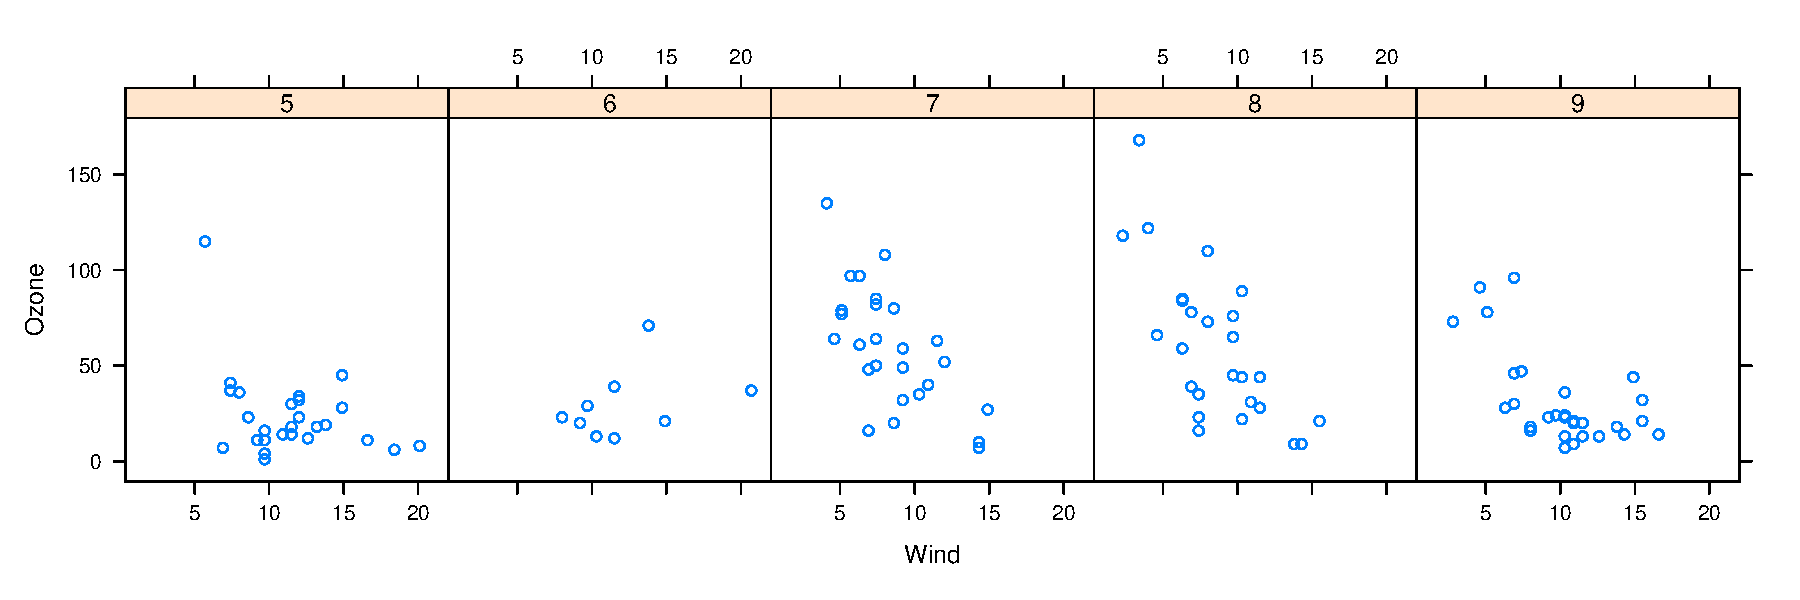
\includegraphics{semana_1_files/figure-latex/unnamed-chunk-2-1} \end{center}

\begin{itemize}
\tightlist
\item
  Encuentra un valor \(C\).
\item
  \textbf{frecuencia de `your' \(>\) C} predice ``spam''
\end{itemize}

\textcolor{red}{patameters}

elegimos un valor de \(c\) de 0.5

\begin{Shaded}
\begin{Highlighting}[]
\FunctionTok{plot}\NormalTok{(}\FunctionTok{density}\NormalTok{(spam}\SpecialCharTok{$}\NormalTok{your[spam}\SpecialCharTok{$}\NormalTok{type}\SpecialCharTok{==}\StringTok{"nonspam"}\NormalTok{]),}
     \AttributeTok{col=}\StringTok{"blue"}\NormalTok{,}\AttributeTok{main=}\StringTok{""}\NormalTok{,}\AttributeTok{xlab=}\StringTok{"Frequency of \textquotesingle{}your\textquotesingle{}"}\NormalTok{)}
\FunctionTok{lines}\NormalTok{(}\FunctionTok{density}\NormalTok{(spam}\SpecialCharTok{$}\NormalTok{your[spam}\SpecialCharTok{$}\NormalTok{type}\SpecialCharTok{==}\StringTok{"spam"}\NormalTok{]),}\AttributeTok{col=}\StringTok{"red"}\NormalTok{)}
\FunctionTok{abline}\NormalTok{(}\AttributeTok{v=}\FloatTok{0.5}\NormalTok{,}\AttributeTok{col=}\StringTok{"black"}\NormalTok{)}
\end{Highlighting}
\end{Shaded}

\begin{center}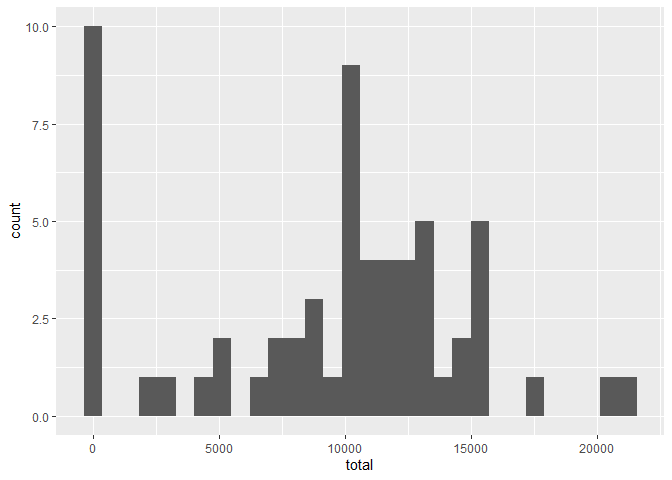
\includegraphics{semana_1_files/figure-latex/unnamed-chunk-3-1} \end{center}

\textcolor{red}{evaluation }

\begin{Shaded}
\begin{Highlighting}[]
\NormalTok{prediction }\OtherTok{\textless{}{-}} \FunctionTok{ifelse}\NormalTok{(spam}\SpecialCharTok{$}\NormalTok{your }\SpecialCharTok{\textgreater{}} \FloatTok{0.5}\NormalTok{,}\StringTok{"spam"}\NormalTok{,}\StringTok{"nonspam"}\NormalTok{)}
\FunctionTok{table}\NormalTok{(prediction,spam}\SpecialCharTok{$}\NormalTok{type)}\SpecialCharTok{/}\FunctionTok{length}\NormalTok{(spam}\SpecialCharTok{$}\NormalTok{type)}
\end{Highlighting}
\end{Shaded}

\begin{verbatim}
##           
## prediction   nonspam      spam
##    nonspam 0.4590306 0.1017170
##    spam    0.1469246 0.2923278
\end{verbatim}

precision \(\approx 0.459 + 0.292 = 0.751\)

\hypertarget{importancia-relativa-de-los-pasos}{%
\section{Importancia relativa de los
pasos}\label{importancia-relativa-de-los-pasos}}

``La combinación de algunos datos y el doloroso deseo de una respuesta
no garantiza que se pueda extraer una respuesta razonable de un conjunto
de datos determinado.''

-John Tukey

\textcolor{red}{input data}

\begin{enumerate}
\def\labelenumi{\arabic{enumi}.}
\tightlist
\item
  Puede ser fácil (clasificaciones de películas -\textgreater{}
  clasificaciones de películas nuevas)
\item
  Puede ser más difícil (datos de expresión genética -\textgreater{}
  enfermedad)
\item
  Depende de lo que sea una ``buena predicción''.
\item
  A menudo, {[}más datos\textgreater{} mejores modelos{]}
  (\url{http://www.youtube.com/watch?v=yvDCzhbjYWs})
\item
  ¡El paso más importante!
\end{enumerate}

¡las características importan!

\textcolor{red}{features}

\textbf{Propiedades de buenas características}

\begin{itemize}
\tightlist
\item
  Conducir a la compresión de datos
\item
  Conservar la información relevante
\item
  Se crean en base al conocimiento de aplicaciones de expertos.
\end{itemize}

\textbf{Errores comunes}

\begin{itemize}
\tightlist
\item
  Intentando automatizar la selección de funciones
\item
  No prestar atención a las peculiaridades específicas de los datos
\item
  Tirar información innecesariamente
\end{itemize}

\textcolor{red}{algorithm}

Los algoritmos importan menos de lo que piensas

Los algoritmos importan menos de lo que piensas, y esto puede ser un una
fuente de sorpresa y frustración para algunas personas. Así que esta es
una tabla en la que intentaron predecir una variedad de diferentes
tareas de predicción, por ejemplo, una especie de tarea de segmentación,
predicción de votos en la Cámara de Representantes de EE. UU., y
predicción de formas de onda y un montón de otras tareas de predicción
diferentes. Y así lo hicieron de dos formas diferentes, primero usaron
algo llamado análisis discriminante lineal que es una especie de un
predictor temprano muy básico que puede aprender. Y luego también
probaron para cada dato configurado para encontrar el mejor algoritmo de
predicción absoluto podrían haberlo hecho y luego esta tabla muestra el
error de predicción de estos dos enfoques diferentes. Y puede ver que el
mejor error de predicción es siempre un poco mejor que el error
discriminante lineal. Pero, en realidad, no está tan lejos.

\begin{center}\includegraphics[width=1\linewidth]{D:/luism/Documents/courses/assets/img/08_PredictionAndMachineLearning/illusiontable} \end{center}

Temas a considerar

\begin{center}\includegraphics[width=1\linewidth]{D:/luism/Documents/courses/assets/img/08_PredictionAndMachineLearning/mlconsiderations} \end{center}

La predicción se trata de compensaciones de precisión

\begin{itemize}
\tightlist
\item
  Interpretabilidad versus precisión
\item
  Velocidad versus precisión
\item
  Simplicidad versus precisión
\item
  Escalabilidad versus precisión (adaptacion)
\end{itemize}

La interpretabilidad importa: declaraciones si / entonces pueden ser muy
interpretables para algunas personas, y esa es la razón por la que a la
gente le gustan cosas como los árboles de decisiones

\hypertarget{error-en-muestra-y-fuera-de-la-muestra}{%
\section{Error en muestra y fuera de la
muestra}\label{error-en-muestra-y-fuera-de-la-muestra}}

\textbf{En Error de muestra}: La tasa de error que obtiene en el mismo
conjunto de datos que usó para construir su predictor. Algunas veces
llamado error de resustitución. (entrenamiento)

\textbf{error fuera de la muestra}: La tasa de error que obtiene en un
nuevo conjunto de datos. A veces se denomina error de generalización.
(prueba)

\textbf{Ideas claves}

\begin{enumerate}
\def\labelenumi{\arabic{enumi}.}
\tightlist
\item
  Lo que le importa es el error fuera de muestra
\item
  En error de muestra \(<\) fuera de error de muestra
\item
  El motivo es el sobreajuste

  \begin{itemize}
  \tightlist
  \item
    Hacer coincidir su algoritmo con los datos que tiene
  \end{itemize}
\end{enumerate}

ejemplo motivacional

\begin{Shaded}
\begin{Highlighting}[]
\FunctionTok{library}\NormalTok{(kernlab); }\FunctionTok{data}\NormalTok{(spam); }\FunctionTok{set.seed}\NormalTok{(}\DecValTok{333}\NormalTok{)}
\NormalTok{smallSpam }\OtherTok{\textless{}{-}}\NormalTok{ spam[}\FunctionTok{sample}\NormalTok{(}\FunctionTok{dim}\NormalTok{(spam)[}\DecValTok{1}\NormalTok{],}\AttributeTok{size=}\DecValTok{10}\NormalTok{),]}
\NormalTok{spamLabel }\OtherTok{\textless{}{-}}\NormalTok{ (smallSpam}\SpecialCharTok{$}\NormalTok{type}\SpecialCharTok{==}\StringTok{"spam"}\NormalTok{)}\SpecialCharTok{*}\DecValTok{1} \SpecialCharTok{+} \DecValTok{1}
\FunctionTok{plot}\NormalTok{(smallSpam}\SpecialCharTok{$}\NormalTok{capitalAve,}\AttributeTok{col=}\NormalTok{spamLabel)}
\end{Highlighting}
\end{Shaded}

\begin{center}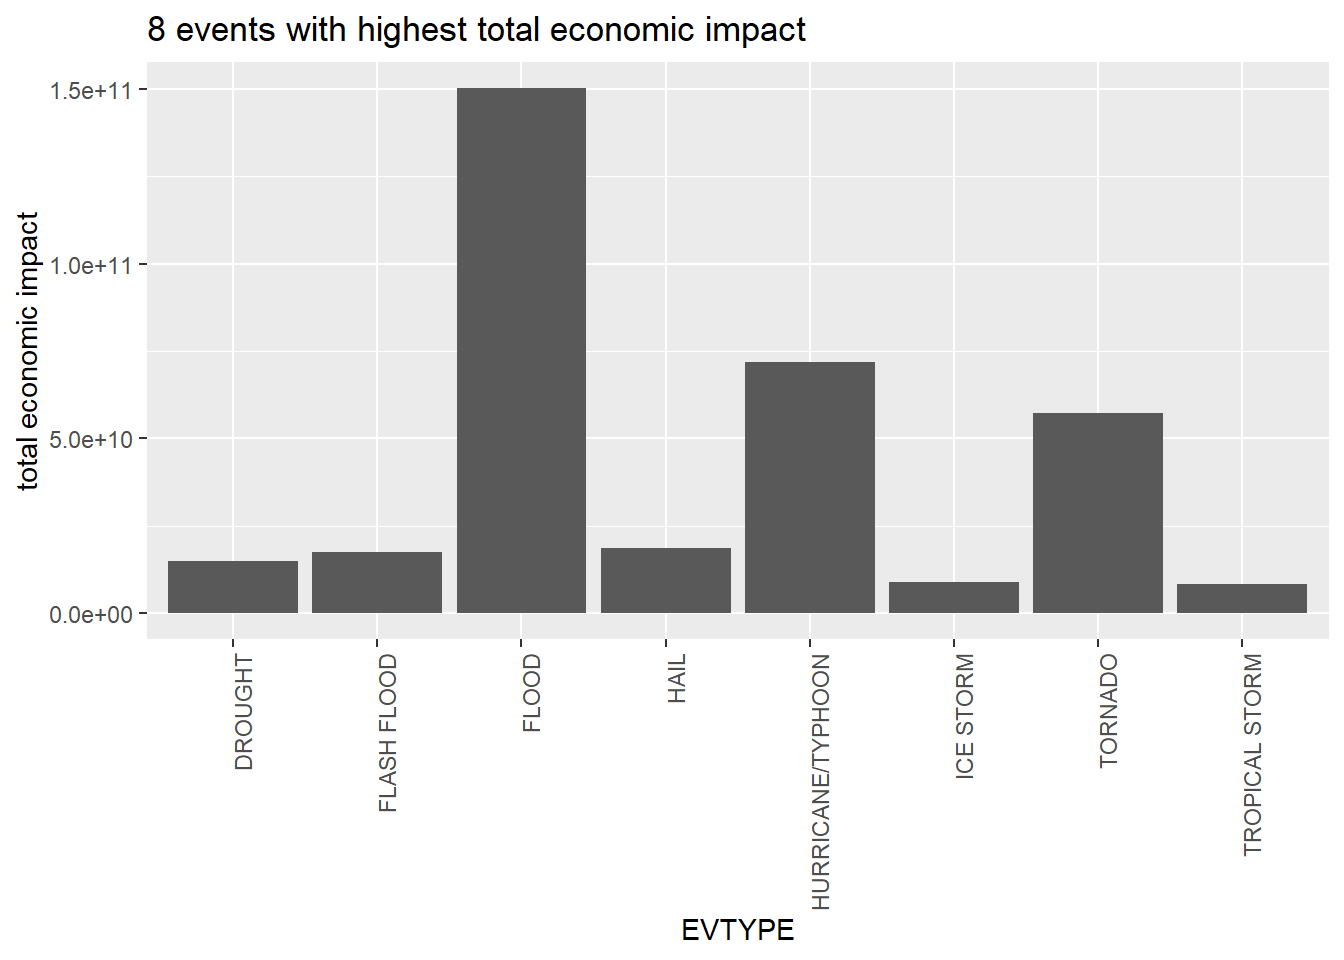
\includegraphics{semana_1_files/figure-latex/unnamed-chunk-7-1} \end{center}

Regla de predicción 1

\begin{itemize}
\tightlist
\item
  capitalAve \(>\) 2.7 = ``spam''
\item
  capitalAve \(<\) 2.40 = ``no spam''
\item
  capitalAve entre 2,40 y 2,45 = ``spam''
\item
  capitalAve entre 2,45 y 2,7 = ``no spam''
\end{itemize}

Aplicando regla de prediccion 1 a smallSpam

\begin{Shaded}
\begin{Highlighting}[]
\NormalTok{rule1 }\OtherTok{\textless{}{-}} \ControlFlowTok{function}\NormalTok{(x)\{}
\NormalTok{  prediction }\OtherTok{\textless{}{-}} \FunctionTok{rep}\NormalTok{(}\ConstantTok{NA}\NormalTok{,}\FunctionTok{length}\NormalTok{(x))}
\NormalTok{  prediction[x }\SpecialCharTok{\textgreater{}} \FloatTok{2.7}\NormalTok{] }\OtherTok{\textless{}{-}} \StringTok{"spam"}
\NormalTok{  prediction[x }\SpecialCharTok{\textless{}} \FloatTok{2.40}\NormalTok{] }\OtherTok{\textless{}{-}} \StringTok{"nonspam"}
\NormalTok{  prediction[(x }\SpecialCharTok{\textgreater{}=} \FloatTok{2.40} \SpecialCharTok{\&}\NormalTok{ x }\SpecialCharTok{\textless{}=} \FloatTok{2.45}\NormalTok{)] }\OtherTok{\textless{}{-}} \StringTok{"spam"}
\NormalTok{  prediction[(x }\SpecialCharTok{\textgreater{}} \FloatTok{2.45} \SpecialCharTok{\&}\NormalTok{ x }\SpecialCharTok{\textless{}=} \FloatTok{2.70}\NormalTok{)] }\OtherTok{\textless{}{-}} \StringTok{"nonspam"}
  \FunctionTok{return}\NormalTok{(prediction)}
\NormalTok{\}}
\FunctionTok{table}\NormalTok{(}\FunctionTok{rule1}\NormalTok{(smallSpam}\SpecialCharTok{$}\NormalTok{capitalAve),smallSpam}\SpecialCharTok{$}\NormalTok{type)}
\end{Highlighting}
\end{Shaded}

\begin{verbatim}
##          
##           nonspam spam
##   nonspam       5    1
##   spam          1    3
\end{verbatim}

Regla de prediccion 2 * capitalAve \(>\) 2.40 = ``spam'' * capitalAve
\(\leq\) 2.40 = ``nonspam''

Aplicando regla de prediccion 2 a smallSpam

\begin{Shaded}
\begin{Highlighting}[]
\NormalTok{rule2 }\OtherTok{\textless{}{-}} \ControlFlowTok{function}\NormalTok{(x)\{}
\NormalTok{  prediction }\OtherTok{\textless{}{-}} \FunctionTok{rep}\NormalTok{(}\ConstantTok{NA}\NormalTok{,}\FunctionTok{length}\NormalTok{(x))}
\NormalTok{  prediction[x }\SpecialCharTok{\textgreater{}} \FloatTok{2.8}\NormalTok{] }\OtherTok{\textless{}{-}} \StringTok{"spam"}
\NormalTok{  prediction[x }\SpecialCharTok{\textless{}=} \FloatTok{2.8}\NormalTok{] }\OtherTok{\textless{}{-}} \StringTok{"nonspam"}
  \FunctionTok{return}\NormalTok{(prediction)}
\NormalTok{\}}
\FunctionTok{table}\NormalTok{(}\FunctionTok{rule2}\NormalTok{(smallSpam}\SpecialCharTok{$}\NormalTok{capitalAve),smallSpam}\SpecialCharTok{$}\NormalTok{type)}
\end{Highlighting}
\end{Shaded}

\begin{verbatim}
##          
##           nonspam spam
##   nonspam       5    1
##   spam          1    3
\end{verbatim}

Aplicar para completar los datos de spam

\begin{Shaded}
\begin{Highlighting}[]
\FunctionTok{table}\NormalTok{(}\FunctionTok{rule1}\NormalTok{(spam}\SpecialCharTok{$}\NormalTok{capitalAve),spam}\SpecialCharTok{$}\NormalTok{type)}
\end{Highlighting}
\end{Shaded}

\begin{verbatim}
##          
##           nonspam spam
##   nonspam    2141  588
##   spam        647 1225
\end{verbatim}

\begin{Shaded}
\begin{Highlighting}[]
\FunctionTok{table}\NormalTok{(}\FunctionTok{rule2}\NormalTok{(spam}\SpecialCharTok{$}\NormalTok{capitalAve),spam}\SpecialCharTok{$}\NormalTok{type)}
\end{Highlighting}
\end{Shaded}

\begin{verbatim}
##          
##           nonspam spam
##   nonspam    2224  642
##   spam        564 1171
\end{verbatim}

\begin{Shaded}
\begin{Highlighting}[]
\FunctionTok{mean}\NormalTok{(}\FunctionTok{rule1}\NormalTok{(spam}\SpecialCharTok{$}\NormalTok{capitalAve)}\SpecialCharTok{==}\NormalTok{spam}\SpecialCharTok{$}\NormalTok{type)}
\end{Highlighting}
\end{Shaded}

\begin{verbatim}
## [1] 0.7315801
\end{verbatim}

\begin{Shaded}
\begin{Highlighting}[]
\FunctionTok{mean}\NormalTok{(}\FunctionTok{rule2}\NormalTok{(spam}\SpecialCharTok{$}\NormalTok{capitalAve)}\SpecialCharTok{==}\NormalTok{spam}\SpecialCharTok{$}\NormalTok{type)}
\end{Highlighting}
\end{Shaded}

\begin{verbatim}
## [1] 0.7378831
\end{verbatim}

Mira la precisión

\begin{Shaded}
\begin{Highlighting}[]
\FunctionTok{sum}\NormalTok{(}\FunctionTok{rule1}\NormalTok{(spam}\SpecialCharTok{$}\NormalTok{capitalAve)}\SpecialCharTok{==}\NormalTok{spam}\SpecialCharTok{$}\NormalTok{type)}
\end{Highlighting}
\end{Shaded}

\begin{verbatim}
## [1] 3366
\end{verbatim}

\begin{Shaded}
\begin{Highlighting}[]
\FunctionTok{sum}\NormalTok{(}\FunctionTok{rule2}\NormalTok{(spam}\SpecialCharTok{$}\NormalTok{capitalAve)}\SpecialCharTok{==}\NormalTok{spam}\SpecialCharTok{$}\NormalTok{type)}
\end{Highlighting}
\end{Shaded}

\begin{verbatim}
## [1] 3395
\end{verbatim}

que esta pasando?(\textcolor{red}{sobreajuste})

\begin{itemize}
\tightlist
\item
  Los datos tienen dos partes

  \begin{itemize}
  \tightlist
  \item
    Señal
  \item
    Ruido
  \end{itemize}
\item
  El objetivo de un predictor es encontrar la señal
\item
  Siempre puede diseñar un predictor perfecto en la muestra
\item
  Capturas tanto la señal como el ruido cuando haces eso
\item
  El predictor no funcionará tan bien en nuevas muestras
\end{itemize}

\url{http://en.wikipedia.org/wiki/Overfitting}

\hypertarget{diseuxf1o-del-estudio-de-predicciuxf3n}{%
\section{Diseño del estudio de
predicción}\label{diseuxf1o-del-estudio-de-predicciuxf3n}}

\begin{enumerate}
\def\labelenumi{\arabic{enumi}.}
\tightlist
\item
  Defina su tasa de error
\item
  Divida los datos en:

  \begin{itemize}
  \tightlist
  \item
    Entrenamiento, Pruebas, Validación
  \end{itemize}
\item
  En el conjunto de entrenamiento, elige caracteristicas.

  \begin{itemize}
  \tightlist
  \item
    Usar validación cruzada
  \end{itemize}
\item
  En la función de predicción de selección del conjunto de entrenamiento

  \begin{itemize}
  \tightlist
  \item
    Usar validación cruzada
  \end{itemize}
\item
  Si no hay validación

  \begin{itemize}
  \tightlist
  \item
    Aplicar 1x al conjunto de prueba
  \end{itemize}
\item
  Si la validación

  \begin{itemize}
  \tightlist
  \item
    Aplicar al conjunto de prueba y refinar
  \item
    Aplicar 1x a la validación
  \end{itemize}
\end{enumerate}

\emph{Evite tamaños de muestra pequeños}

Reglas generales para el diseño de estudios de predicción

\begin{itemize}
\tightlist
\item
  Si tiene un tamaño de muestra grande

  \begin{itemize}
  \tightlist
  \item
    60\% de formación
  \item
    Prueba del 20\%
  \item
    20\% de validación
  \end{itemize}
\item
  Si tiene una muestra de tamaño medio

  \begin{itemize}
  \tightlist
  \item
    60\% de formación
  \item
    40\% de prueba
  \end{itemize}
\item
  Si tiene un tamaño de muestra pequeño

  \begin{itemize}
  \tightlist
  \item
    Hacer validación cruzada
  \item
    Informe de advertencia de tamaño de muestra pequeño
  \end{itemize}
\end{itemize}

\emph{algunos principios para recordar}

\begin{itemize}
\tightlist
\item
  Deje a un lado la prueba / validación y \emph{no lo mire}
\item
  En general, muestra de entrenamiento y prueba son \emph{aleatorios}
\item
  Sus conjuntos de datos deben reflejar la estructura del problema

  \begin{itemize}
  \tightlist
  \item
    Si las predicciones evolucionan con el entrenamiento/prueba dividido
    en el tiempo en fragmentos de tiempo (llamado {[}backtesting{]}
    (\url{http://en.wikipedia.org/wiki/Backtesting}) en finanzas)
  \end{itemize}
\item
  Todos los subconjuntos deben reflejar la mayor diversidad posible

  \begin{itemize}
  \tightlist
  \item
    La asignación aleatoria hace esto
  \item
    También puede intentar equilibrar por características, pero esto es
    complicado
  \end{itemize}
\end{itemize}

\hypertarget{tipos-de-error}{%
\section{Tipos de error}\label{tipos-de-error}}

\hypertarget{para-resultados-binarios}{%
\subsection{para resultados binarios}\label{para-resultados-binarios}}

En general, \textbf{Positivo} = identificado y \textbf{negativo} =
rechazado. Por lo tanto:

\textbf{Verdadero positivo} = identificado correctamente

\textbf{False positivo} = identificado incorrectamente

\textbf{Verdadero negativo} = correctamente rechazado

\textbf{False negative} = rechazado incorrectamente

\emph{Ejemplo de prueba médica}:

\textbf{Verdadero positivo} = Personas enfermas correctamente
diagnosticadas como enfermas

\textbf{Falso positivo } = Personas sanas identificadas incorrectamente
como enfermas

\textbf{Verdadero negativo} = Personas sanas correctamente identificadas
como sanas

\textbf{False negative} = Personas enfermas incorrectamente
identificadas como saludables.

\begin{itemize}
\tightlist
\item
  \emph{La sensibilidad} (tasa de verdaderos positivos) mide la
  proporción de positivos que se identifican correctamente (es decir, la
  proporción de aquellos que tienen alguna afección (afectados) que se
  identifican correctamente como portadores de la afección).
\item
  \emph{La especificidad} (tasa de verdaderos negativos) mide la
  proporción de negativos que se identifican correctamente (es decir, la
  proporción de aquellos que no tienen la afección (no afectados) que se
  identifican correctamente como personas que no padecen la afección).
\end{itemize}

\begin{center}\includegraphics[width=1\linewidth]{D:/luism/Documents/courses/assets/img/keyquantities} \end{center}

\begin{center}\includegraphics[width=1\linewidth]{D:/luism/Documents/courses/assets/img/keyquantfrac} \end{center}

Ahora pongamos un ejemplo: Suponga que alguna enfermedad tiene una
prevalencia del 0,1\% en la población. Supongamos que tenemos un kit de
prueba para esa enfermedad que funciona con una sensibilidad del 99\% y
una especificidad del 99\%. ¿Cuál es la probabilidad de que una persona
tenga la enfermedad dado que el resultado de la prueba es positivo, si
seleccionamos al azar un sujeto de

\begin{itemize}
\tightlist
\item
  la población en general?
\item
  una subpoblación de alto riesgo con una prevalencia de enfermedad del
  10\%?
\end{itemize}

Población general

\begin{center}\includegraphics[width=1\linewidth]{D:/luism/Documents/courses/assets/img/predpos2} \end{center}

Población general como fracciones

\begin{center}\includegraphics[width=1\linewidth]{D:/luism/Documents/courses/assets/img/predpos3} \end{center}

Subpoblación en riesgo

\begin{center}\includegraphics[width=1\linewidth]{D:/luism/Documents/courses/assets/img/predpos4} \end{center}

Subpoblación en riesgo como fracciones

\begin{center}\includegraphics[width=1\linewidth]{D:/luism/Documents/courses/assets/img/predpos5} \end{center}

\hypertarget{para-el-caso-continuo}{%
\subsection{para el caso continuo}\label{para-el-caso-continuo}}

\textbf{Error cuadrático medio(MSE) }:

\[\frac{1}{n}\sum_{i = 1}^n(Predicción_i-Verdad_i)^2\]

\textbf{Raíz de el error cuadrático medio (RMSE) }:

\[\sqrt{\frac{1}{n}\sum_{i = 1}^n (Predicción_i - Verdad_i) ^ 2}\]

\hypertarget{medidas-de-error-comunes}{%
\subsection{Medidas de error comunes}\label{medidas-de-error-comunes}}

\begin{enumerate}
\def\labelenumi{\arabic{enumi}.}
\tightlist
\item
  Error cuadrático medio (o error cuadrático medio)

  \begin{itemize}
  \tightlist
  \item
    Datos continuos, sensibles a valores atípicos
  \end{itemize}
\item
  Desviación absoluta mediana

  \begin{itemize}
  \tightlist
  \item
    Datos continuos, a menudo más robustos
  \end{itemize}
\item
  Sensibilidad (recuerdo)

  \begin{itemize}
  \tightlist
  \item
    Si quieres pocos positivos perdidos
  \end{itemize}
\item
  Especificidad

  \begin{itemize}
  \tightlist
  \item
    Si quieres algunos negativos llamados positivos
  \end{itemize}
\item
  Precisión

  \begin{itemize}
  \tightlist
  \item
    Pondera los falsos positivos / negativos por igual
  \end{itemize}
\item
  Concordancia

  \begin{itemize}
  \tightlist
  \item
    Un ejemplo es {[}kappa{]}
    (\url{http://en.wikipedia.org/wiki/Cohen\%27s_kappa})
  \end{itemize}
\item
  Valor predictivo de un positivo (precisión)

  \begin{itemize}
  \tightlist
  \item
    Cuando está revisando y el predominio es bajo
  \end{itemize}
\end{enumerate}

\hypertarget{caracteruxedstica-operativa-del-receptor-curvas}{%
\section{Característica Operativa del Receptor
(curvas)}\label{caracteruxedstica-operativa-del-receptor-curvas}}

\begin{itemize}
\tightlist
\item
  En la clasificación binaria está prediciendo una de dos categorías

  \begin{itemize}
  \tightlist
  \item
    Vivo muerto
  \item
    Haga clic en el anuncio / no haga clic
  \end{itemize}
\item
  Pero tus predicciones suelen ser cuantitativas

  \begin{itemize}
  \tightlist
  \item
    Probabilidad de estar vivo
  \item
    Predicción en una escala del 1 al 10
  \end{itemize}
\item
  El \emph{cutoff} que elijas da resultados diferentes
\end{itemize}

La curva ROC , es un diagrama gráfico que ilustra la capacidad de
diagnóstico de un sistema clasificador binario a medida que varía su
umbral de discriminación. El método fue desarrollado originalmente para
operadores de receptores de radar militares a partir de 1941, lo que
llevó a su nombre.

La curva ROC se crea trazando la tasa de verdaderos positivos (TPR)
frente a la tasa de falsos positivos (FPR) en varios valores de umbral

\begin{center}\includegraphics[width=1\linewidth]{D:/luism/Documents/courses/assets/img/08_PredictionAndMachineLearning/roc2} \end{center}

\begin{center}\includegraphics[width=1\linewidth]{D:/luism/Documents/courses/assets/img/08_PredictionAndMachineLearning/roc1} \end{center}

\begin{itemize}
\tightlist
\item
  AUC = 0.5: adivinación aleatoria
\item
  AUC = 1: clasificador perfecto
\item
  En general, el AUC superior a 0,8 se considera ``bueno''
\end{itemize}

\begin{center}\includegraphics[width=1\linewidth]{D:/luism/Documents/courses/assets/img/08_PredictionAndMachineLearning/roc3} \end{center}

\hypertarget{validacion-cruzada}{%
\section{Validacion Cruzada}\label{validacion-cruzada}}

\hypertarget{enfoque-1}{%
\subsection{enfoque 1}\label{enfoque-1}}

\begin{enumerate}
\def\labelenumi{\arabic{enumi}.}
\tightlist
\item
  La precisión en el conjunto de entrenamiento (precisión de
  resustitución) es optimista
\item
  Una mejor estimación proviene de un conjunto independiente (precisión
  del conjunto de prueba)
\item
  Pero no podemos usar el conjunto de prueba al crear el modelo o se
  convierte en parte del conjunto de entrenamiento.
\item
  Por tanto, estimamos la precisión del conjunto de prueba con el
  conjunto de entrenamiento.
\end{enumerate}

\emph{Acercarse}:

\begin{enumerate}
\def\labelenumi{\arabic{enumi}.}
\item
  Usa el conjunto de entrenamiento
\item
  Divídalo en conjuntos de entrenamiento/prueba
\item
  Construya un modelo en el conjunto de entrenamiento.
\item
  Evaluar en el equipo de prueba
\item
  Repetir y promediar los errores estimados
\end{enumerate}

\emph{Usado para}:

\begin{enumerate}
\def\labelenumi{\arabic{enumi}.}
\item
  Seleccionar variables para incluir en un modelo
\item
  Elegir el tipo de función de predicción que se utilizará
\item
  Seleccionar los parámetros en la función de predicción
\item
  Comparación de diferentes predictores
\end{enumerate}

Diferentes formas de dividir los datos

\begin{enumerate}
\def\labelenumi{\arabic{enumi}.}
\tightlist
\item
  Random subsampling
\end{enumerate}

\begin{center}\includegraphics[width=1\linewidth]{D:/luism/Documents/courses/assets/img/08_PredictionAndMachineLearning/random} \end{center}

Este método consiste al dividir aleatoriamente el conjunto de datos de
entrenamiento y el conjunto de datos de prueba. Para cada división la
función de aproximación se ajusta a partir de los datos de entrenamiento
y calcula los valores de salida para el conjunto de datos de prueba. El
resultado final se corresponde a la media aritmética de los valores
obtenidos para las diferentes divisiones. La ventaja de este método es
que la división de datos entrenamiento-prueba no depende del número de
iteraciones. Pero, en cambio, con este método hay algunas muestras que
quedan sin evaluar y otras que se evalúan más de una vez, es decir, los
subconjuntos de prueba y entrenamiento se pueden solapar

\begin{enumerate}
\def\labelenumi{\arabic{enumi}.}
\setcounter{enumi}{1}
\tightlist
\item
  K-fold
\end{enumerate}

\begin{center}\includegraphics[width=1\linewidth]{D:/luism/Documents/courses/assets/img/08_PredictionAndMachineLearning/kfold} \end{center}

Se dividen en K subconjuntos. Uno de los subconjuntos se utiliza como
datos de prueba y el resto (K-1) como datos de entrenamiento. El proceso
de validación cruzada es repetido durante k iteraciones, con cada uno de
los posibles subconjuntos de datos de prueba. Finalmente se realiza la
media aritmética de los resultados de cada iteración para obtener un
único resultado. Este método es muy preciso puesto que evaluamos a
partir de K combinaciones de datos de entrenamiento y de prueba, pero
aun así tiene una desventaja, y es que, a diferencia del método de
retención, es lento desde el punto de vista computacional

\begin{enumerate}
\def\labelenumi{\arabic{enumi}.}
\setcounter{enumi}{2}
\tightlist
\item
  Leave one out
\end{enumerate}

\begin{center}\includegraphics[width=1\linewidth]{D:/luism/Documents/courses/assets/img/08_PredictionAndMachineLearning/loocv} \end{center}

Implica separar los datos de forma que para cada iteración tengamos una
sola muestra para los datos de prueba y todo el resto conformando los
datos de entrenamiento. La evaluación viene dada por el error, y en este
tipo de validación cruzada el error es muy bajo, pero en cambio, a nivel
computacional es muy costoso, puesto que se tienen que realizar un
elevado número de iteraciones, tantas como N muestras tengamos y para
cada una analizar los datos tanto de entrenamiento como de prueba.

\textbf{Consideraciones}

\begin{itemize}
\tightlist
\item
  Para los datos de series de tiempo, los datos deben usarse en
  ``fragmentos''
\item
  Para validación cruzada de k-fold

  \begin{itemize}
  \tightlist
  \item
    Mayor k = menos sesgo, más varianza
  \item
    Más pequeño k = más sesgo, menos varianza
  \end{itemize}
\item
  El muestreo aleatorio debe realizarse \emph{sin reemplazo}
\item
  El muestreo aleatorio con reemplazo es el \emph{bootstrap}

  \begin{itemize}
  \tightlist
  \item
    Subestima el error
  \item
    Se puede corregir, pero es complicado ({[}0.632 Bootstrap{]}
    (\url{http://www.jstor.org/discover/10.2307/2965703?uid=2\&uid=4\&sid=21103054448997}))
  \end{itemize}
\item
  Si realiza una validación cruzada para elegir la estimación de
  predictores, debe estimar los errores en datos independientes.
\end{itemize}

\hypertarget{enfoque-2}{%
\subsection{enfoque 2}\label{enfoque-2}}

cuando hacemos validacion cruzada desde el enfoque 1 existe la
posibilidad de que pase el mismo efecto en el conjunto de prueba que el
que pasa en el conjunto de entrenamiento, es decir que que haya un
sobreajuste generado por el conjunto de prueba

Para solucionar esto, podemos introducir un tercer conjunto, el Conjunto
de validación cruzada , para que sirva como conjunto intermedio.
Entonces, nuestro conjunto de prueba nos dará un error preciso y no
optimista.

Una forma de ejemplo de dividir nuestro conjunto de datos en tres
conjuntos es:

\begin{itemize}
\tightlist
\item
  Conjunto de entrenamiento: 60\%
\item
  Conjunto de validación cruzada: 20\%
\item
  Equipo de prueba: 20\%
\end{itemize}

Ahora podemos calcular tres valores de error separados para los tres
conjuntos diferentes.

\begin{enumerate}
\def\labelenumi{\arabic{enumi}.}
\tightlist
\item
  Optimice los parámetros en \(\Theta\) utilizando el conjunto de
  entrenamiento.
\item
  Encuentre el menor error usando el conjunto de validación cruzada.
\item
  Estime el error de generalización usando el conjunto de prueba (si es
  muy grande hay un sobreajuste)
\end{enumerate}

\hypertarget{varianza-vs-sesgo}{%
\section{varianza vs Sesgo}\label{varianza-vs-sesgo}}

\hypertarget{en-estadistica}{%
\subsection{En estadistica}\label{en-estadistica}}

El \emph{sesgo} mide lo lejos que se encuentra el valor estimado
respecto al real de la población completa. Por ejemplo, si se desea
calcular la vida media de unas bombillas es necesario escoger una
muestra. El tiempo de vida promedio de esta muestra es el que se le
asocia a la población, pero no tiene porque se el de la población total.
Este error es lo que se llama como sesgo.

Al trabajar con una muestra aleatoria de la población total es de
esperar que sea diferente de otra muestra. Esta diferencia entre las
muestras es lo que la ´\emph{varianza}. Así cada vez que se realiza un
nuevo muestreo se observa que los resultados suelen ser diferentes.

\hypertarget{en-machine-learning}{%
\subsection{En Machine learning}\label{en-machine-learning}}

\emph{sesgo}

En aprendizaje automático para estimar un valor se utilizan modelos.
Existiendo muchas familias entre los que escoger. Por ejemplo, en un
problema de clasificación se puede utilizar regresiones logísticas o
random forest entre otros. Pero no todos los modelos son iguales, ya que
cada uno presenta diferentes propiedades.

Así que una pregunta obvia es cómo se relaciona cada una de las familias
de modelos con el sesgo de las predicciones. El sesgo habitualmente
presenta una relación inversa con la complejidad de los modelos. Es
decir, a mayor complejidad del modelo utilizado es de esperar una menor
sesgo.

Ahora bien, ¿qué se entiende por complejidad de un modelo? Por ejemplo,
la regresión logística es un modelo más simple que un árbol de decisión.
La regresión logística asume cierta relación entre las características y
el valor a predecir. Por otro lado, random forest es más complejo en el
sentido de que utiliza un conjunto de árboles de decisión para realizar
las predicciones.

\emph{varianza}

El entrenamiento de los modelos se realiza con conjuntos de dato
diferentes sobre los que posteriormente se utiliza para validar las
predicciones. A los que se conocen como conjunto de entrenamiento y test
respectivamente. Por este hecho es de esperar que ambos conjuntos sean
ligeramente diferentes. Es importante tener en cuenta que cuando entrena
a un modelo no se esperar que este memorice los valores, sino que
encuentre patrones. Observándose en muchas ocasiones que modelos
complejos ajustan bien a los datos de entrenamiento, pero no sucede lo
mismo con los de validación. En donde se suele observar que fallan.

La varianza también se puede relacionar con la complejidad de los
modelos. A medida que aumenta la complejidad, aumentan las posibilidades
de sobreajuste, es decir, la varianza aumenta. Al comparar la regresión
logística con random forest se espera que la varianza del primero se
meno que la del segundo

\begin{itemize}
\tightlist
\item
  El sesgo alto es desajuste y la varianza alta es sobreajuste.
\item
  se trata de encontrar un equilibrio entre el sesgo, varianza
\end{itemize}

\hypertarget{recursos}{%
\section{recursos}\label{recursos}}

\begin{itemize}
\tightlist
\item
  \href{http://statweb.stanford.edu/~tibs/ElemStatLearn/}{The elements
  of statistical learning}
\item
  \href{http://www.quora.com/Machine-Learning/What-are-some-good-resources-for-learning-about-machine-learning-Why}{List
  of machine learning resources on Quora}
\item
  \href{http://www.sciencemag.org/site/feature/data/compsci/machine_learning.xhtml}{List
  of machine learning resources from Science}
\item
  \href{http://ocw.mit.edu/courses/electrical-engineering-and-computer-science/6-867-machine-learning-fall-2006/lecture-notes/}{Advanced
  notes from MIT open courseware}
\item
  \href{http://www.stat.cmu.edu/~cshalizi/350/}{Advanced notes from CMU}
\item
  \href{http://www.kaggle.com/}{Kaggle - machine learning competitions}
\item
  \href{http://en.wikipedia.org/wiki/Receiver_operating_characteristic}{ROC}
\end{itemize}

\end{document}
